\begin{frame}{File formats: VCF}

Tab delimited text file with a \textbf{header section}

\begin{figure}[htbp]
\centering
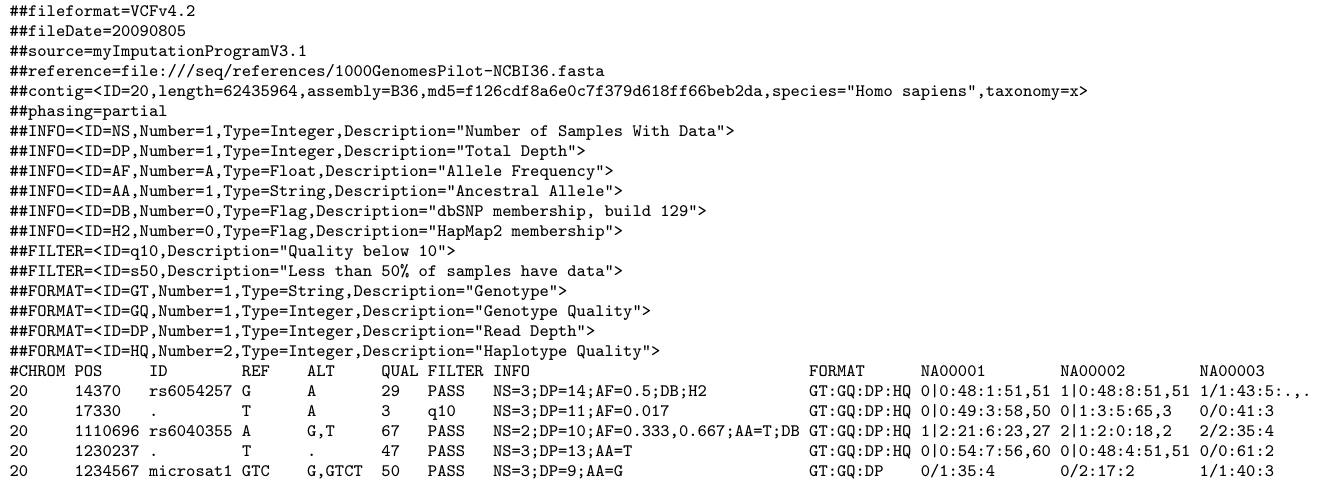
\includegraphics[width=\textwidth,height=0.8\textheight,keepaspectratio]{images/vcf.png}
\end{figure}

May be compressed and indexed using \texttt{tabix}

\end{frame}

\begin{frame}{File formats: VCF}

Each variant is described by \textbf{8 fields}

\begin{enumerate}
\def\labelenumi{\arabic{enumi}.}
\item
  CHROM: chromosome
\item
  POS: position
\item
  ID: name
\item
  REF: reference base(s)
\item
  ALT: non-reference alleles
\item
  QUAL: quality score of the calls (phred scale)
\item
  FILTER: PASS / filtering\_tag
\item
  INFO: additional information
\end{enumerate}

\textbf{Genotype data} for several samples may be included in a batch of
additional columns (one for each sample) preceded by a FORMAT column
which describes their format.

\end{frame}

\begin{frame}[fragile]{File formats: VCF INFO column}

May include several semicolon separated fields containing information
about the variants coded in key value style:

\begin{verbatim}
<key>=<data>[,data]
\end{verbatim}

Some reserved (but optional) keys are:

\begin{itemize}
\itemsep1pt\parskip0pt\parsep0pt
\item
  AA ancestral allele
\item
  AC allele count in genotypes, for each ALT allele, in the same order
  as listed
\item
  AF allele frequency
\item
  CIGAR cigar string describing how to align an alternate allele to the
  reference allele
\item
  DB dbSNP membership
\item
  MQ RMS mapping quality, e.g.~MQ=52
\item
  MQ0 Number of MAPQ == 0 reads covering this record
\end{itemize}

\end{frame}

\begin{frame}{File formats: PED \& MAP}

Classic format to represent genomic variants for several individuals

\centerline{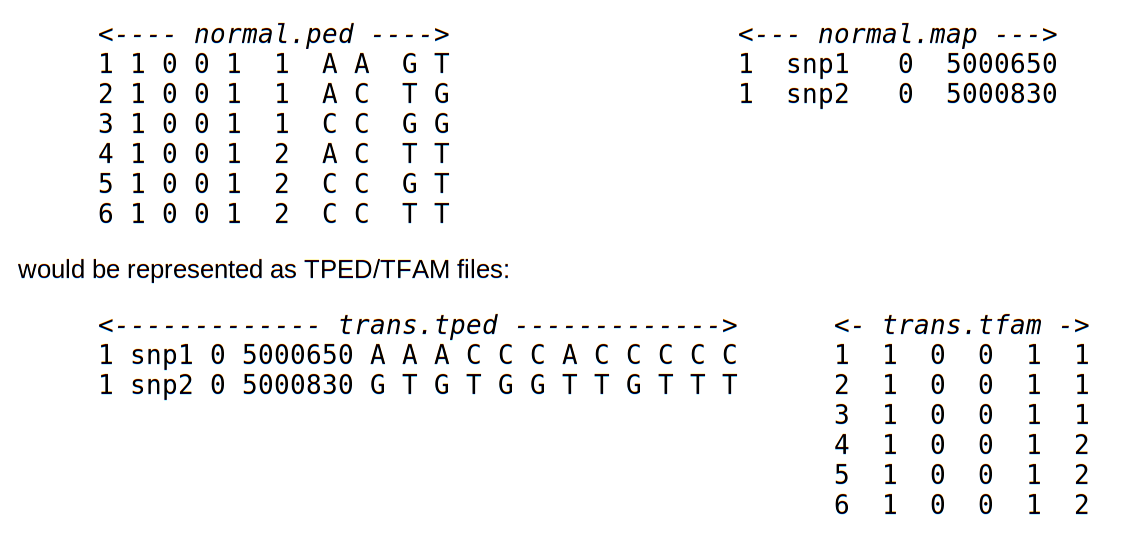
\includegraphics[scale=0.3]{images/ped-map.png}}

\small

Some variants of the format are described depending on the software used
to read or write them. Those variants may include \emph{transposed}
versions of the format which is closer to standard \emph{genomic}
representation of this kind of information.

\end{frame}

\begin{frame}{File formats: PED \& MAP}

\begin{block}{PED file}

\begin{enumerate}
\def\labelenumi{\arabic{enumi}.}
\itemsep1pt\parskip0pt\parsep0pt
\item
  Family ID
\item
  Individual ID
\item
  Paternal ID
\item
  Maternal ID
\item
  Sex (1=male; 2=female; other=unknown)
\item
  Phenotype (1=unaffected; 2=affected; 0 missing; -9=missing)
\item
  \ldots{} genotypes \ldots{}
\end{enumerate}

\end{block}

\begin{block}{MAP file}

\begin{enumerate}
\def\labelenumi{\arabic{enumi}.}
\itemsep1pt\parskip0pt\parsep0pt
\item
  chromosome (1-22, X, Y or 0 if unplaced)
\item
  rs\ldots{} or SNP identifier
\item
  Genetic distance (Morgans)
\item
  Base-pair position (bp units)
\end{enumerate}

\end{block}

\end{frame}
